% This is samplepaper.tex, a sample chapter demonstrating the
% LLNCS macro package for Springer Computer Science proceedings;
% Version 2.20 of 2017/10/04
%
\documentclass[runningheads]{llncs}
%
\usepackage{graphicx}
\usepackage{cite}
\usepackage{svg}


% Used for displaying a sample figure. If possible, figure files should
% be included in EPS format.
%
% If you use the hyperref package, please uncomment the following line
% to display URLs in blue roman font according to Springer's eBook style:
% \renewcommand\UrlFont{\color{blue}\rmfamily}

\begin{document}
%
\title{Extracting Points of Interest from Geospatial Data with KNIME}
%
%\titlerunning{Abbreviated paper title}
% If the paper title is too long for the running head, you can set
% an abbreviated paper title here
%
\author{L. Mandruzzato \and
A. Weikert}
%
\authorrunning{Mandruzzato \& Weikert}
% First names are abbreviated in the running head.
% If there are more than two authors, 'et al.' is used.
%
\institute{ISTIC, Université de Rennes 1, Beaulieu - Bâtiment 12D, \\263 Avenue du Général Leclerc, 35042 Rennes, France \\ \email{leonardo.mandruzzato@etudiant.univ-rennes1.fr} \email{alexander.weikert@etudiant.univ-rennes1.fr}}
%
\maketitle              % typeset the header of the contribution
%
\begin{abstract}
This paper analyzes geospatial data from Flickr. It aims to extract points of interest to improve the public transport system of Rennes, France. Firstly, we cluster the data based on the coordinates only. Then, we use a text processing pipeline to extract the bag of words from the dataset. In doing so, we cluster the data again based on both coordinates and captions and compare both models. Lastly, we characterize the points by searching for frequent itemsets within the captions.

\keywords{Geospatial data \and Social Media Data \and Clustering \and Frequent Itemset \and Bag of Words (BoW)}
\end{abstract}
%
%
%
\section{Introduction}\label{intro}
We have been given a data set containing mainly the geodata, timestamp, and caption of several thousand photos uploaded to social media. Our assignment is to automate the discovery and characterization of points of interest to improve the public transport system of the city of Rennes. A point of interest is "defined by the presence of a substantial amount of pictures." This report documents the steps we took to achieve that goal.

There is no codebook that restrains the analytic capability of this paper. Furthermore, the domain knowledge is limited to our private use of social media, i.e., we make assumptions about the industry. We will make notes wherever domain knowledge could help to improve the results.

This paper is organized as follows. Section \ref{data} introduces the data set and describes its characteristics. Also, data cleaning and preparation are explained. Section \ref{analysis} documents the approach and results for discovering and characterizing points of interest. Section \ref{finalRemarks} gives a perspective for possible future work.

Lastly, this paper is part of the final grading of the 2021 fall semester lecture "Data Mining (FSY, M2 Miage BDDA + EIT)" at the Rennes 1 University in France held by Sébastien Ferré.

\section{Data}\label{data}
The following section gives an overview of the data set and its characteristics. Furthermore, it reports the cleaning and pre-processing measures being used.

\subsection{Data set}
The given data set originates from the social media platform Flickr. For the sake of this assignment, we assume the source of the data and its collection process to be credible despite the missing codebook.

The data frame contains 54\,800 rows and 14 columns, namely the photographer ID, longitude and latitude, photo ID, tags (as in hashtag), photo title, and lastly, date and time, stored in 8 different columns.

\subsection{Data preparation}\label{data preparation}
Our task is to discover points of interest in the city of Rennes, i.e., to cluster the given data. We present the approach and results in section \ref{analysis}. To get there, we must prepare the data first. We were mainly facing dirty data.

Dirty data can appear due to duplicate values, misspellings, data type parsing errors, and legacy systems \cite{dirty_data}. However, only character encoding errors, misspellings, and duplicate values caught our attention after changing the timestamp's data type.

Let us tackle the duplicates first. For example, all photos were taken between 1987 and 2017. The 19th of March 2017 alone contains 31\,925 rows, i.e., 58.26\% of the data. All rows from said date contain the same photographer ID (137920363@N03), title (La Rennaise 2017), and coordinate (48.139179, -1.641232). The coordinate leads to the stadium Robert Launay in Rennes. The timestamps range from 08:46:39 to 12:14:16. To conclude, we can link all features to the running event La Rennaise \cite{athle}.

However, from the 31\,925 rows, there are only 1\,560 unique photo IDs. We are not Flickr users, but we assume that there are indeed only 1\,560 unique photos, but users shared them several times, and with each share, the system writes a duplicate of the shared photo's tuple. Here, a domain expert is needed.

There are several approaches to tackle duplicates. Since we cannot verify whether a duplicate means the same photo has been shared several times or whether there is another explanation, we choose to exclude all photo ID duplicates. Keeping them seems negligent to us. The database decreases to 4\,195 rows.

After tackling the duplicates, we set the character set for the encoding type to UTF-8. In doing so, French characters, especially, e.g., à, á, â, are displayed correctly. Regarding misspellings, we only observe them in the columns tags and title, which are fields filled by the social media user manually. It is well known that social media text is noisy \cite{becker_2009, java_2007} as cited in \cite{baldwin_2013}. In conclusion, we need to treat social media text very carefully. To do so, we focus on three main tasks: scraping data (get words from titles and tags), filtering the irrelevant terms, and finally computing the bag-of-words (BoW) model.

Apart from the trivial components used to erase the punctuation, delete numbers and short words, and put everything in lower case, the most interesting part is the one used for removing redundant terms and lemmatizing the remaining ones. To remove redundant tags, we passed the default English and French lists of words to the "Stop Word Filter" \cite{stop_word_lists}. In addition, we wrote a list containing some irrelevant terms like Rennes, France, Ille-et-Vilaine, and many others that do not carry any information. Regarding the lemmatizing task, we used the predefined node named "Stanford Lemmatizer". However, it considers only English words and not French ones. Therefore, we preferred the lemmatizer instead of a "Snowball Stemmer" because the results with the latter would be hard to analyze for a non-native French speaker.

Lastly, we experiment with feature engineering and selection. We normalize the coordinates. We also notice that all unique photo IDs correspond to one unique coordinate. Therefore, a performance comparison between two different data sets was not possible.

\section{Points of interests}\label{analysis}
\subsection{Discovery}\label{clustering}
In this section, we discover points of interest to improve the public transport system of the city of Rennes. A point of interest is "defined by the presence of a substantial amount of pictures".

\begin{figure}
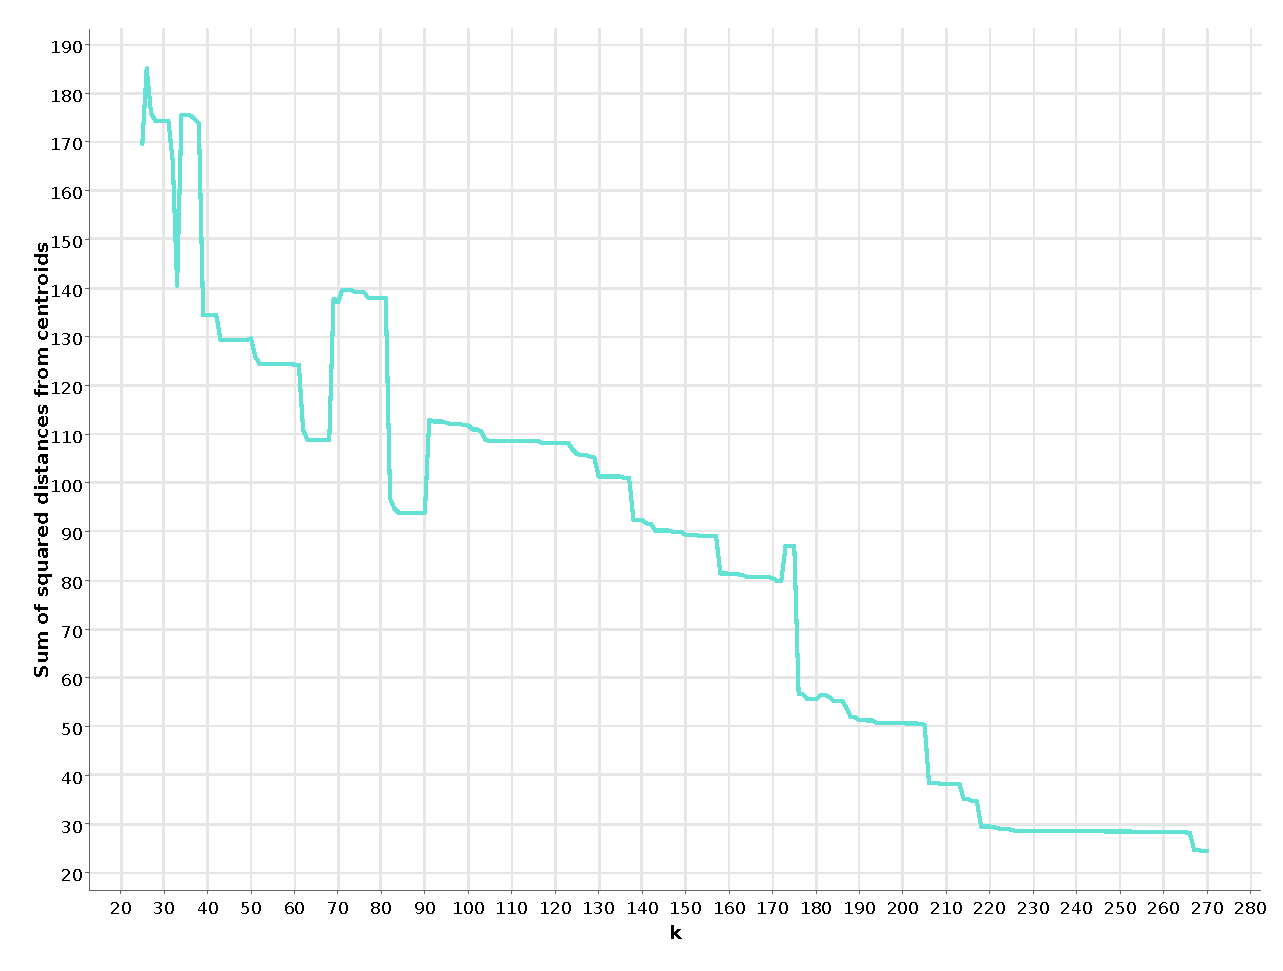
\includegraphics[width=\textwidth]{elbowAnalysis_4195_coordinates.eps}
\caption{Elbow analysis of k-Means with coordinates only} \label{elbow_coordinates}
\end{figure}

For our baseline, we use a k-Means model considering only the coordinates. Figure~\ref{elbow_coordinates} shows the elbow analysis of the said model. For each {\itshape k}, we can see the sum of the squared distances to the cluster's centroid. There is no intuitive optimum. However, there are several interesting points we would like to discuss. For example, at $k$ equal to 39, 63, 83, 176, and 218, the sum of squared distances rapidly decreases. However, before most of those points, the sum of squared distances also significantly increased.

Figure~\ref{mapViewsFor2k} shows the map view of both extremes, $k=39$ and $k=218$. Please note that we used color coding for the colorblind. So, the bigger yellow area on the left of the second photo consists of three different clusters.

To conclude, there is no intuitive $k$. With a smaller $k$, we can see popular neighborhoods. This could be used to plan routes for public transport roughly. With a bigger $k$, we can detect popular points within a neighborhood to plan the exact positions for bus stops. Nevertheless, the clusters need to be characterized first. Also, domain experts are needed to interpret the results more deeply.

\begin{figure}
\centering
\includegraphics[width=6cm]{k=39.png}
\includegraphics[width=6cm]{k=218.png}
\caption{Map view for k-Means with $k=39$ (left) and $k=218$ (right)} \label{mapViewsFor2k}
\end{figure}

After introducing a naive model that considers coordinates only, we implemented a second model that additionally utilizes the bag of words. For example, an event close to the decision boundary can be torn into two different clusters. After including the title and tag features, we can obtain a model more sensitive to the user input. Unfortunately, it is computationally costly to optimize $k$. Therefore, we randomly experimented with different values of $k$. Without the elbow curve and without further characterization, it is not very meaningful to compare the results between these two models.

\subsection{Characterization}\label{leonardo}
In the previous section, we discovered points of interest and gave the first possibility to interpret the results. However, the results are not fully interpretable before further characterization.

To do so, we use a text processing pipeline to characterize the discovered clusters to extract words and tags from each picture. Then, we search for the ones that appear repetitively inside each cluster and characterize them - i.e., the frequent itemsets.

Ideally, we can split the designed pipeline into two parts. One, to obtain the bag of words - i.e., BoW - of the dataset (see section \ref{data preparation}). The other, to find the frequent itemsets.

\subsubsection{Frequent itemsets research}
Analyzing our Knime model and, specifically, the portion of it related to the frequent itemsets discovery, it's easily guessable how we approached this problem from the presence of a cycle. We did not search for them in the whole dataset and then linked the results to the clusters - e.g., through association rules. We instead looked for frequent itemsets cluster by cluster. We tried both solutions, and there are no differences in the results apart from better readability of the ones obtained through the second method.

We noticed an enormous impact of the {\itshape k} value on the research success for frequent itemsets. The higher is the number of clusters, the fewer pictures will be inside each of them. The less data we have, the less reliable the results we will obtain. For instance, if a cluster contains only four pictures and one of them has a specific tag, the support of that word would be 25\%, even if the term is meaningless. In our case, already with {\itshape k} equal to 40, we fail to find frequent itemsets with support higher than 10\% among all the different points of interest. Moreover, the ones we get are often meaningless and useless to characterize that group of photos. Thus, to increase {\itshape k} and do a more detailed analysis, we need more data.

\subsubsection{Split of the pipeline}
Initially, we used the whole text processing pipeline - i.e., BoW creation + Frequent Itemsets research - after the clustering analysis, with the sole purpose of characterizing the obtained points of interest. Although the two parts belong to the same workflow, we split them and anticipated the BoW model's one. In this way, we exploited the latter and its associated document vector to improve clustering (see section \ref{clustering}).

\subsubsection{Results}
Analyzing the tags/words obtained, we managed to get reasonable results.  Let' us start comparing the differences between the outcomes obtained from k-Means and k-Medoids when $k=30$.  With k-means, photos that share the same tags and have similar coordinates may be included in 2 different clusters. Shouldn't they be a single cluster? Since this method only considers coordinates, it may be that it detects two groups of photos. If there is a vast point of interest characterized by the same tags - e.g., a park - the algorithm may split it into two clusters (see first two rows of Table \ref{tab1}). 
Moreover, if two points of interest have similar coordinates, the k-Means algorithm creates a single group containing all of them. And that is reasonable, but it does not consider the possibility of having photos with similar positions but with completely different tags (see last two rows of Table \ref{tab1}).
All of this does not happen with k-Medoids. In some ways, this method is more effective and precise, making the characterization work easier. In the end, its results are more focused (see Table \ref{tab2}).

Now, we can move on to the actual characterization of the clusters by making some examples and referring to Table \ref{tab3}. We can start making some general considerations by looking at those recurrent words among the different clusters. For instance, street arts and graffiti in Rennes seem to be of interest and thus definitely attractive for tourists. Moreover, it is possible to find suggestive views around the city, especially in parks and during foggy seasons.

Focusing on tags belonging to only one cluster, we can spot the most famous places in Rennes like Parc Thabor or Palais Saint-Georges. It is possible to spot also the group of pictures belonging to the event "La Rennaise 2017". Furthermore, it is possible to go deeper and find some niche places like Écomusée de la Bintinais, and sometimes some cafes/clubs like Le Cartel Loco (unfortunately closed permanently).

In the context of our task – to improve the public transportation system – we need more domain knowledge. For example, is street art illegal in Rennes and more likely to change in an unforeseeable pattern, or is it supported by the administration and even under protection? For the former, changing the public transport system is too costly, but it could be worth it for the latter. Domain knowledge is also helpful when discovering local cafes and clubs. Unfortunately, we do not know which bar is famous already and which is not. We can imagine that some establishments are frequented at certain times, which could significantly impact the schedule density. Also, will La Rennaise reoccur in the future or will it remain an event in 2017 only?

\begin{table}
\caption{Table with an excerpt of the frequent itemsets obtained after a k-Means analysis with $k=30$. It could be noticed how almost identical itemsets are shared between different clusters (first 2 rows). And we can observe how pictures with very different tags may be in the same grouping (last 2 rows).}\label{tab1}
\begin{tabular}{|p{7cm}|c|c|l|}
\hline
\textbf{ItemSet} &  \textbf{Support} & \textbf{Rel. Support} & \textbf{Cluster}\\
\hline
art, street, porte, quai, mabilais, door, collectif, sculpteur, belge, telecom, happen, wale, peche, asphalt, fisher, zephyr, saintcyr, boomer, captain, echouage, baleine, cachalot, tour & 18 & 8.18\% & cluster\_29\\
\hline
art, cachalot, mabilais, street, baleine, tour, porte, quai, captain, boomer, saintcyr, peche, wale, happen, belge, fisher, sculpteur, collectif, door, zephyr, telecom, asphalt, echouage & 19 & 16.81\% & cluster\_1\\
\hline
 jerkovmusique,  live, parpaing, noise, postrock, mathrock, loud, indie, luikrecord, jerkov, design, yaof, yaofdesign, concert, lysistrata, cartel, loco, paleblueskin, idealcrash, lecartelloco & 22 & 19.47\% & cluster\_1\\
\hline
\end{tabular}
\end{table}

\begin{table}
\caption{Table with an excerpt of the frequent itemsets obtained after a k-Medoids analysis with $k=30$. If we observe the relative supports and compare them with the ones of Table \ref{tab1}, we immediately get how this clusterization is more effective. There are no more different clusters with same itemsets, neither same clusters with different tags.}\label{tab2}
\begin{tabular}{|p{7cm}|c|c|l|}
\hline
\textbf{ItemSet} &  \textbf{Support} & \textbf{Rel. Support} & \textbf{Cluster}\\
\hline
art, cachalot, mabilais, baleine , street, tour, saintcyr, boomer, captain, quai, belge, sculpteur, collectif, happen, door, porte, zephyr, fisher, asphalt, peche, wale, telecom, echouage & 37 & 35.57\% & Row3341\\
\hline
concert, design, yaof, yaofdesign, live, jerkov, parpaing, noise, postrock, mathrock, loud, indie, luikrecord, jerkovmusique, lecartelloco, idealcrash, paleblueskin, loco, cartel, lysistrata & 22 & 38.59\% & Row1272\\
\hline
\end{tabular}
\end{table}

\begin{table}
\caption{Table with an excerpt of the frequent itemsets obtained after k-Means analysis with $k=30$.}\label{tab3}
\begin{tabular}{|p{7cm}|c|c|l|}
\hline
\textbf{ItemSet} &  \textbf{Support} & \textbf{Rel. Support} & \textbf{Cluster}\\
\hline
\textbf{rennaise} & 1560 & 100\% & cluster\_16\\
\hline
\textbf{thabor}, parc & 33 & 25.98\% & cluster\_20\\
\hline
\textbf{thabor}, jardin & 13 & 10.24\% & cluster\_20\\
\hline
goudron, \textbf{graphitis}, \textbf{street}, \textbf{art}, tag, escalier, batiment, \textbf{saintgeorge}, build, travaux, graph, pasteur, chantier, door, stair, porte, park, hotel, palai, dentaire, asphalte, fresque, panneaux, bitume, fac, scooter, vespa & 6 & 8.11 & cluster\_2\\
\hline
\textbf{ecomusee}, tournesol, horse, farm, machine, garden, fruit, legume, vegetable, veggy, wool, sheep, mouton, chevre, ble, sleep, endormi, lait, milk, cow, vache, ferme, medaille, elevage, jument, duck, barrel, tonneau, chil, enfant, caractere, printer, cat, vilaine, canard, land, pay, cheval, jardin, ille, chat, champ, imprimerie, monotype, linotype, typographue, oberthur, expo & 67 & 80.72 & cluster\_7\\
\hline
 jerkovmusique,  live, parpaing, noise, postrock, mathrock, loud, indie, luikrecord, jerkov, design, yaof, yaofdesign, concert, lysistrata, cartel, loco, paleblueskin, idealcrash, \textbf{lecartelloco} & 22 & 19.47\% & cluster\_1\\
\hline
\textbf{street}, \textbf{art}, build, batiment, egout, porte, door, goudron, panneaux, asphalte, fresque, bitume, \textbf{graphitis}, graph, tag, sale, pave & 27 & 9.06 & cluster\_21\\
\hline
street, hiver, asphalt, building, manege, foraine, bruine, beton, bitume, apparition, \textbf{foggy}, fair, carrousel, fete, fantome, \textbf{brume}, \textbf{fog}, \textbf{brouillard}, parc, fun, attraction, esplanade, foire & 57 & 35.19 & cluster\_26\\
\hline
\end{tabular}
\end{table}

\section{Final Remarks}\label{finalRemarks}
We can observe the potential of this kind of analysis. With a small quantity of data - i.e., 4\,195 pictures - and a basic model, it is already possible to find meaningful results. However, if we combine more data with more advanced models to run the same analysis, the findings could be substantial. Even more if domain experts - e.g., Rennes Tourism Office employees - analyze the results to extract information.

For further analysis on the technical side, we would include the photo captions for the clustering part already. Finding the optimal $k$ takes more computational power, which should not be a problem in a real-life scenario. We could pay for the Amazon Web Service, for example. Furthermore, we could use more clustering techniques, e.g., hierarchical, density-based, or fuzzy clustering.

For further knowledge extraction, we would differentiate between points that are interesting all year round and points that are interesting only on certain days. Are the latter repetitive or an outlier? We would also differentiate between the city center and suburbs. The distance to the centroids outside of the city is much larger. Hence, they may need a different model. All of the approaches above can be crucial to adjust the public transportation system.

However, the influence of tourists on the public transport system is, by all means, not a one-way street but works in both ways. Therefore, every change in the system must be validated and compared in a preferably isolated way. To conclude, this is not a process that happens from one day to the other, but more of an infinite process, and this analysis is only one tool out of many.

%
% ---- Bibliography ----
%
% BibTeX users should specify bibliography style 'splncs04'.
% References will then be sorted and formatted in the correct style.
%
% \bibliographystyle{splncs04}
% \bibliography{mybibliography}
%
\begin{thebibliography}{8}
\bibitem{baldwin_2013}
Baldwin, T., Cook, P., Lui, M., MacKinlay, A., Wang, L. (2013, October). How noisy social media text, how differnt social media sources?. In Proceedings of the Sixth International Joint Conference on Natural Language Processing (pp. 356-364).

\bibitem{becker_2009}
Becker, H., Naaman, M., Gravano, L. (2009). Event identification in social media. In Proceedings of the 12th International Workshop on the Web and Databases (WebDB 2009), Providence, USA.

\bibitem{athle}
Fédération Française d'Athlétisme. (2017). La Rennaise 2017. \url{http://aspttrennes.athle.com/asp.net/espaces.html/html.aspx?id=35931}

\bibitem{java_2007}
Java, A. (2007). A framework for modeling influence, opinions and structure in social media. In Proceedings of the 22nd Annual Conference on Artificial Intelligence (AAAI-07), pages 1933–1934.

\bibitem{stop_word_lists}
Knime. (2018, October). Stop Word Lists., \url{https://github.com/knime/knime-textprocessing/tree/master/org.knime.ext.textprocessing.models/stopwordlists}

\bibitem{dirty_data}
Wu, J. (2019, October 2). What is Dirty Data?. \url{https://towardsdatascience.com/what-is-dirty-data-d96abbdf254e}.
\end{thebibliography}
\end{document}
